\chapter{Vocal Accommodation in Real-World Sales Calls}
\label{chap:conv_analysis}

\lettrine{H}{uman}-human interaction is an essential part of sales representatives' everyday work.
Controlling their communication skills is key for their deal to be successful.
The role of vocal accommodation in measuring and improving said skills is presented here as part of the greater concept of \acl{c-iq}.
The analyses use non-linear methods to examine mutual influences in a collection of real-world high-stake sales calls.

\pagebreak

\section{Speech alignment for conversation intelligence}
\label{sec:conversation_intelligence}

Sales leaders have always been impelled to be able to reason why some of their representatives -- henceforth \emph{reps} or \emph{\acp{ae}} -- consistently attain, or even exceed, their goals while others do not \citep[see overview in][]{Kovac2017its}.
Yet, sales executives rely on data that is inherently flawed, as it is based on reports from sources like \ac{crm} systems.
Such systems only contain \enquote{dry} details regarding the stage the deals are in along with high-level numeric data and some, often subjective, estimations regarding the next steps.
That leaves the executives in the dark about the happenings at the front lines and the small-scale, day-to-day conducts and modi operandi that are decisive for the success of the \acp{ae}.
As a result, the reasons for losing or winning a deal often remain a riddle, making sales seem like an art based on anecdotes rather than a scientifically explainable practice \citep{Yohn2016best, Martin2017six}.
In his seminal book, \citet{Gladwell2006tipping} writes that \textquote[p.\ 83]{Part of what it means to have a persuasive personality is that you can draw others into your own rhythms and dictate the terms of the interaction}.
Supporting that, \citet{Orlob2018nine} found that star reps\footnote{Sales representative whose performances (and specifically their closed-deals rate) are often refer to as \emph{star reps}.The specific criteria are typically include a wide range of behavioral and business metrics, but those are decided internally per company and do not have an absolute definition.} are able to make prospects increase their speaking rate to match theirs, bringing the two sides closer with respect to this phonetic feature.
However, the scientific analysis is far from the everyday work, and such phenomena are passed on as general tips and are never taught or explained in detail to the \acp{ae}.
\Ac{c-iq} systems aim to bridge over this gap and connect the scientific side of sales to the field, to help reps improve their performance using measured, interpretable methods they can learn from.

Here, the focus is on another phonetic feature, namely \ac{f0}.
This feature can be interpreted and explained by people with little or no phonetic training, like \acp{ae}.
Furthermore, it can be easily controlled by speakers, making it a tangible tool for the \acp{ae} to exploit to improve their performance, as opposed to, e.g., more complex, acoustic features like \acp{mfcc} or changes in the \ac{ltas} that are often used in phonetic accommodation studies \citep{Levitan2011measuring, Borrie2019syncing}.
For this, a large-scale corpus of real-world conversations was used, which takes the examination of phonetic accommodation out of the controlled, supervised experimental laboratory environment.
The conversations in this corpus are therefore mostly flexible and structured-free than experiments in laboratory setting (like those in \cref{chap:shadowing_experiment_with_natural_and_synthetic_voices}), as there are no instructions or defined tasks to perform.
By extension, they are also more authentic and spontaneous, since the interlocutors are driven solely by their own behavior and motivation to succeed and are not given a temporary role to fill as part of an experiment.
\Ac{crqa} \citep{Zbilut1998detecting}, a bivariate correlation technique, is used for the analysis.
This method finds instances where coordinates of two time series occur close to each other within a certain radius in some phase-space continuum.
Since \ac{crqa} can evaluate the degree to which the similarity of two time series changes over time, and can also determine the leading relationship between them, it is highly suitable and informative for analyzing phonetic accommodation between two speakers.
A comprehensive overview of this method is presented by \citet{Wallot2018analyzing}, and the way it is used here is explained in \cref{sec:crqa}.
The contributions of this study are therefore both in methodology of measuring accommodation and its practical application in a real-world purpose.

\subsection{\Acl{c-iq}}
\label{subsec:conversation_intelligence}

There are influences on the way we communicate and structure to how conversations unfold.
These can be analyzed and interpreted to uncover conversation-level trends, which may differ from the linear, turn-by-turn changes.
\Acf{c-iq} is a relatively newly coined term and a field of research that flourished due to advancements in neuroscience, communication science, and \ac{ml}.
It complements other types of human intelligence (e.g., \emph{emotional intelligence}, and c.f.\ \emph{Theory of Multiple Intelligences} \citep{Gardner1983frames, Davis2011theory}) as the ensemble of aspects conversations are handled \textbf{beyond the surface words and shared information}.
\citet{Glaser2016conversational} explains and demonstrates how \ac{c-iq} can be learned and improved, with emphasis on the ability to gain trust and maintain more successful and healthy communication with others.
\todo{add 1-2 key ideas from the book?}
Although \ac{c-iq} comprises many further aspects beyond the scope of this work, the overarching idea of improvable communication between people by changing one's communication behavior is highly relevant in the context of vocal accommodation, which is seldom used for such analyses.

Narrowing down this broad idea, \citet{SilberVarod2018human} discusses the way individual conversations can be \emph{managed}.
This includes both the structure and evolution of a conversation over time and the dynamics of the interlocutors' roles in it.
Noticeably, it concludes that some speech-related phenomena in conversations tend to be more complex and unpredictable than how it might seem from their surface form.
One of those phenomena is phonetic entrainment.
Such works dealing with managing spoken interactions become even more relevant with the growing interest in intelligent conversational systems for civilian purposes as well \citep{Mehr2017artificial}.
Recently, the importance of \ac{c-iq} has pervaded the enterprise sector and created new businesses.
Specifically, the utilization of computer-based customer services \citep{Gnewuch2017towards} and conversation intelligence services for inside sales calls to train representatives and improve performance \citep{Orlob2017winning,Orlob2017separates}).
It was found, for example, that distinguished sales reps let the prospects talk more and keep certain parts of the calls shorter than others.

\subsection{Inside sales}
\label{subsec:inside_sales}

In recent years, many companies have adopted the concept of \emph{inside sales}, where \ac{b2b} sales are done using web-based conferencing solutions, as opposed to face-to-face meetings with the clients.
Recent technological advancements allow automatic recording and transcription of inside sales calls, aggregating large-scale datasets.
These datasets include the audio of the calls and sometimes annotations such as the call success or the rating of the \ac{ae}.
Inside sales deals have a typical process:
First, a \ac{sdr} reaches out to a potential client (the \emph{prospect}) who has expressed interest in the company's product.
This creates a \emph{lead}.
Subsequently, the \ac{sdr} shares basic details about the product and how it can help the prospect.
Finally, if the \ac{sdr} has managed to elicit initial interest, the lead turns into an \emph{opportunity}, and a demo call with a sales representative is scheduled.
Such demo calls are often done using a web conferencing tool, such as Zoom\footnote{\url{https://zoom.us}} or GoToMeeting\footnote{\url{https://www.gotomeeting.com}}, which allows both sides to share their webcams and screens.
Such a dataset is analyzed in this work (see \cref{sec:dataset_calls}).
Since these calls were made as a first step after the prospect expressed interest in the company's product, it can be assumed that the behavior and verbal skills of the \ac{ae} will have a larger weight in the success of the call than in calls that may fail due to lack of interesting in the product from the prospect's side.

\subsection{Speaker roles and influences}
\label{subsec:speaker_roles_and_influences}

Although \ac{c-iq} doesn't traditionally use accommodation measures for evaluation as mentioned above, there has been some attempts to use the former for the latter's benefit.
\citet{Glaser2016conversational} explains how important it is that speakers in a business conversation are aligned on the turn level.
Lack of of alignment can result in a skeptic and even resisting behavior that will worsen the quality and success change of the call (cf.\ Table 2 in \citet{Glaser2014conversational}).
At the very least, this demonstrates how important it is, as a whole, for interlocutors to be attentive not only to the contents but also to the way the communication is conveyed during a conversation (and in sales call, for the sales rep in particular).
\citet{SilberVarod2018human} shows how vocal convergence is related to power relations aspects in \ac{c-iq} analyses.
Specifically, speaker \enquote{dominancy} is sometimes hard to spot on the surface but becomes more clear when examining the vocal relations between the speakers.
Analyses like this improve the the understanding of vocal behaviors in \ac{hhi}.
Furthermore, \citet{Abrego2011effects} discusses how judgment of speaker's role in a conversation influences on phonetic aspects of production.
The idea of speakers' behavioral modifications due to their role and perception of the other interlocutor is a key concept for the presented study.

\section[\Acl{crqa}]{\Acl{crqa} for measuring accommodation}
\label{sec:crqa}

Depending on the circumstances, \ac{hhi} may involve different communication modalities, such as facial expression, hand gestures, eye gaze, and more.
The analyses here concentrate on the phonetic level, as it is the primary modality used for conveying information in sales calls, even if video or screen sharing are available as well.
It has been shown in various studies based on \ac{cat} \citep[][and cf.\ \cref{sec:communication_accommodation_theory}]{Giles1991CAT, Gallois2015CAT} that humans naturally tend to change their speech behavior within a conversation based on the speech they hear from another human speaker \citep[see, e.g.][]{Bailly2010speech, Babel2014novelty}.
Such mutual adjustment in \ac{hhi} also increases the success of the conversation \citep{Pickering2004behavioral} and affects the social distance between speakers \citep{Schweitzer2017social}.
Accordingly, effects of the same nature have been found in sales calls as well, as presented in \cref{subsec:speaker_roles_and_influences}.

Linear methods for measuring accommodation rely on the chronological, turn-by-turn order of the interaction.
These methods are limited to detection of local phenomena evolving gradually across adjacent turns.
See \cref{subsec:limitations_of_did,fig:accommodation_types} for more details about the limitations of using \ac{did} for measuring accommodation.
Non-linear methods, on the other hand, are not dependent on the chronological order of the interaction's turn and can therefore find long-term, more distant relations between the speakers with respect to a defined target feature.
For instance, that an accommodation process (or generally closer values) occurred at some point in the beginning and continued at a later time, or that there was a periodic pattern of convergence and divergence throughout the interaction.
Such phenomena point to more general, conversation-level properties that do not rely on the chronological unfolding order of the turns.
This is especially useful for long interaction, like sales calls tend to be, where a more general view may be insightful.
The conversations in the large-scale corpus used here (see \cref{sec:dataset_calls}) have an inherent structure and are considerably longer than in typical experimental setups.
This encourages the use of \ac{crqa} to quantify the accommodation over the course of whole conversations to detect long-term relations and accommodation structures, instead of comparing two halves of the conversation or neighboring turns, as often done \citep{Levitan2013entrainment,Rahimi2018weighting}.
Such analyses overlook the serial temporal nature of such \acp{hhi}, which falls under the definition of a \emph{time series}.
This open a new variety of non-linear methods that can enhance accommodation analysis
Non-linear analysis methods for time series include, among others, noise reduction and non-linear prediction, e.g., for finance and natural phenomena.
The method utilized here uses phase-space embedding, which describes temporal evolution of trajectories of a dynamic system by projecting their embedding onto some common space.

\subsection{Capturing different behaviors with \acs{crqa}}
\label{subsec:capturing_behaviors}

In this study, the target features are either evaluated when detected or sampled in defined intervals using a dedicated system for accommodation analysis \citep[][and see details in \cref{sec:dataset_calls}]{Raveh2018Specom}.
Furthermore, these values are extracted in chronological order, and thus produce sequences of discrete-time data, which makes them suitable for time series-based analysis.
Due to the nature of these features (and perhaps any spontaneous, interactive linguistic feature), the resulted time series can be assumed to be non-seasonal and non-stationary.
%\todo{make sure that saying that doesn't invalidates the use of CRQA}
This recognition as time series opens new methodological possibilities for examining the evolution of these features and their realizations by different speakers in an interaction over time.
Such methods include, for example, autocorrelation for examining serial dependency and forecasting for transferring information about the time series across time.
These methods can extend upon others in analyzing accommodation, with the advantage of offering more dynamic approach rather than the sequential methods usually used.

One such analysis method is \acf{crqa}, which provides insights on the time series across an entire time span (here, a conversation).
This is done by comparing delayed instances of the phase-space trajectories of time series.
This allows finding more general patterns in the time series characteristics and how they interact.
It is especially suitable for studying accommodation and related phenomena, as it detect times in which the time series (i.e., the speakers' productions) are more similar.
Moreover, it can mathematically show which of the time series led the alignment or whether the changes were done in synchrony (see overview of these processes in \cref{subsec:variation_types}).
Is has already been used in \ac{hhi} research.
For instance, for analyzing and predicting differences in scenarios with disagreement and deceptive behavior \citep{Duran2017conversing}.
Similar method was used to measure conversational entrainment for assessing speech pathology \citep{Borrie2019syncing}, finding that sessions in which periods of synchronization were established were rated as more successful by therapists.
This is a good example of a cooperative interaction with a common goal where accommodation unconsciously contributes this its success.
In sum, \ac{crqa} can be used to objectively quantify and describe accommodation between speakers dynamically across entire conversations.
\Cref{subsec:recurrence_detection,subsec:parameters_crqa} explain the technicalities of \ac{crqa}, how its output can be interpreted, and how it is used in the studies presented here.

\begin{figure}[H]
	\centering
	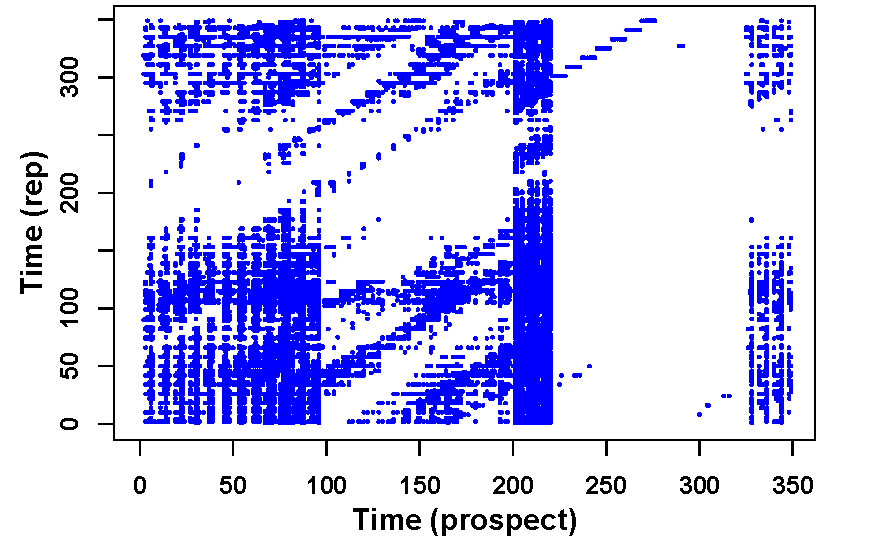
\includegraphics[width=\linewidth]{crqa_plot_115993376241473405}
	\caption[\acs{crqa} analysis of pitch in a sales call]
		{A recurrence plot generated for one of the analyzed conversations.
		The y-axis marks the conversation timeline, in time stamp, of the \ac{ae}, and the x-axis of the prospect.
		Each blue dot represents a co-visitation of a similar state.
		Blue dots forming an diagonal line indicate sustained recurrence between the two speakers (see description of NRLINE in \cref{subsec:output_values} for details).
		Note that the time stamps on the axes are not the slices, but the embedded call time.
		For example, the diagonal structures between time stamps 100 and 200 of the x-axis show such lasting recurrence.
		Diagonal lines above the \acl{los} (\acs{los}; the central diagonal line) indicate that the speaker on the y-axis leads the x-axis, and vice versa for lines below the \ac{los}.
		The blank area between time stamps 220 and 330 of the x-axis point to a portion of the call where the speakers were more distant from each other.}
	\label{fig:crqa_plot}
	\todo[inline]{make the plot square, to make it clearer that the times have the same length}
\end{figure}

\subsection{Recurrence detection}
\label{subsec:recurrence_detection}

\Ac{rqa} is a non-linear analysis method that quantifies the number and duration of recurrences withing a dynamical system presented by its state-space trajectory, which is typically the realization of a sampled time series.
It was introduced by \citet{Zbilut1992embeddings} and later extended by \citet{Webber2005recurrence, Marwan2002cross}.
A \emph{recurrence} (also, \emph{re-visitation}) is a time in which the trajectory returns to a state (or a similar-enough state, as explained below) it has visited before.
Recurrence can therefore be defined as the binary function

\begin{equation}
	\label{eq:recurrence}
	R_{i,j} =
	\begin{cases}
		1,	&	\text{if} \quad \lVert \vec{x}(i)-\vec{x}(j) \rVert_d \leq \varepsilon \\
		0,	&	\text{otherwise} \\
	\end{cases},
\end{equation}
%
where $i$ and $j$ are x-axis and y-axis coordinates in a recurrence plot (see \cref{fig:crqa_plot}), respectively, $d$ are the embedding dimensions, and $\varepsilon$ defines the threshold distance below which two cross-trajectory points are considered similar (see explanation about the \emph{radius} parameter in \cref{subsec:parameters_crqa}).
In a recurrence plot, the points $R_{i,j}$ are colored equal if their value is 1 or stay white otherwise.
\Ac{crqa} is an extension of \ac{rqa} analyzing recurrence quantification between two different time series rather than a single one time series with itself.
As such, \ac{crqa} is a quantification technique for non-linear dynamical systems that describes when and to what extent concurrences (or \emph{co-visitations}) can be found in a system consists of two time series.
These quantification techniques are based on \emph{recurrence plots} that for each moment $i$ in time show the times at which a phase space trajectory visits roughly the same area in the phase space as at time $i$.
Ultimately, a recurrence plot is a graph of $\vec{x}(i) \approx \vec{x}(j)$, showing $i$ on the x-axis and $j$ on the y-axis, where $\vec{x}$ is a phase space trajectory (see example in \cref{fig:crqa_plot}).
\todo[inline]{maybe take one of the RPs from the website and add the LoS (and other diagonals) to it to provide more detailed visualization?}
Each colored point in the plot represents a time where the time series were close to each other based on the definition in \cref{eq:recurrence}.
The main diagonal of the plot is called the \acf{los}.
A high number of recurrences along this line indicates synchrony between the time series.
However, diagonal recurrence lines can be formed above and below the \ac{los}.
Such diagonals, especially longer ones, represent delayed (lagged) synchrony between the time series and can be used as an assessment of similarity between the processes.
In the context of accommodation, these diagonals imply an accommodative change led by one of the interlocutors.
If the diagonal stretches above the \ac{los}, the speaker plotted on the x-axis leads the accommodation, and vice versa.
The closer the diagonal is from the \ac{los}, the quicker the process occurred, i.e., the led speaker aligned his behavior to the leading speaker after a shorter time.
Due to its ability to detect these similarities non-linearly, \ac{crqa} can be utilized to measure accommodation in the scope of entire conversations rather than taking only neighboring turns into account \citep[cf.][]{Levitan2013entrainment}.

\subsection{Parameter tuning}
\label{subsec:parameters_crqa}

\Ac{crqa} uses three parameters:

\begin{enumerate}
	\item \textbf{Delay} -- estimates the temporal shift required to make the two time series maximally aligned.
	It is measured by the same time unit as the time series, in the presented studies, a slice (see \cref{subsec:results_hhi}).
	
	\item \textbf{Embedding dimensions} -- are the number of dimensions into which the data points are embedded.
	These dimensions are delayed copies of the original time series $S(t)$ created by adding a lag $k$ to them.
	Typically, multiple lags are considered, which create the dimensions of embedding $S(t + nk)$.
	
	\item \textbf{Radius} -- determines the margin within which two data points are considered a recurrent instance.
	Distances between the data points are measured in the embedded space defined by embedding dimensions, using the same unit used for measuring the values of the time series.
\end{enumerate}
%
These parameters are a crucial key aspect in \ac{crqa} and how they are set is decisive for its outcome.
However, although some best-practice guidelines, like those suggested by \citet{Coco2014crqa-r}, exist, there is nevertheless no standard way for optimizing these parameters, especially due to the fact that they depend on the nature and characteristics of the data.
A method similar to the one presented by \citet{Marwan2007recurrence} was utilized in the analysis presented here.
The delay parameter was determined by finding the lag that minimizes the average mutual information between the two time series, which is determined by
%
% from https://www.frontiersin.org/articles/10.3389/fpsyg.2018.01679/full
\begin{equation}
	\label{eq:average_mutual_information}
	I\left( x(t), x(t + \tau) \right) = \sum_{i,j} p_{ij} (\tau) \log \left( \frac{p_{ij} \left( \tau \right)}{p_i p_j} \right).
\end{equation}
\eqname{Average mutual information (AMI)}
%
This provides a delay that is not too short to miss the different distributions, but also not too long to lose the dependency between the time series.
The lag with the \emph{lowest} average mutual information was selected, regardless of when the values started to level off.
Subsequently, the number of embedding dimensions was obtained using false nearest neighbors \citep{Kennel1992determining}.
This algorithm determines the minimum embedding dimension necessary to reconstruct the state space of a dynamical system with time delay embedding \citep{Abarbanel1993local}.
A neighborhood diameter equal to the standard deviation of the time series was used, and a limit of 20 embedding dimensions (which was never reached) was set.
\Cref{fig:ami,fig:false_nn} show examples of mutual information and false nearest neighbors optimizations.
%
\begin{figure}[H]
	\centering
	\begin{minipage}{.45\linewidth}
		\centering
		\includegraphics[width=\linewidth]{ami}
		\caption
		[Average mutual information of time series as function of lag]
		{The average mutual information of the time series values as a function of the lags considered.
			The x-axis shows the considered lags and the y-axis the mutual information index (AMI) in bits.}
		\label{fig:ami}
	\end{minipage}%
	\hfill
	\begin{minipage}{.45\linewidth}
		\centering
		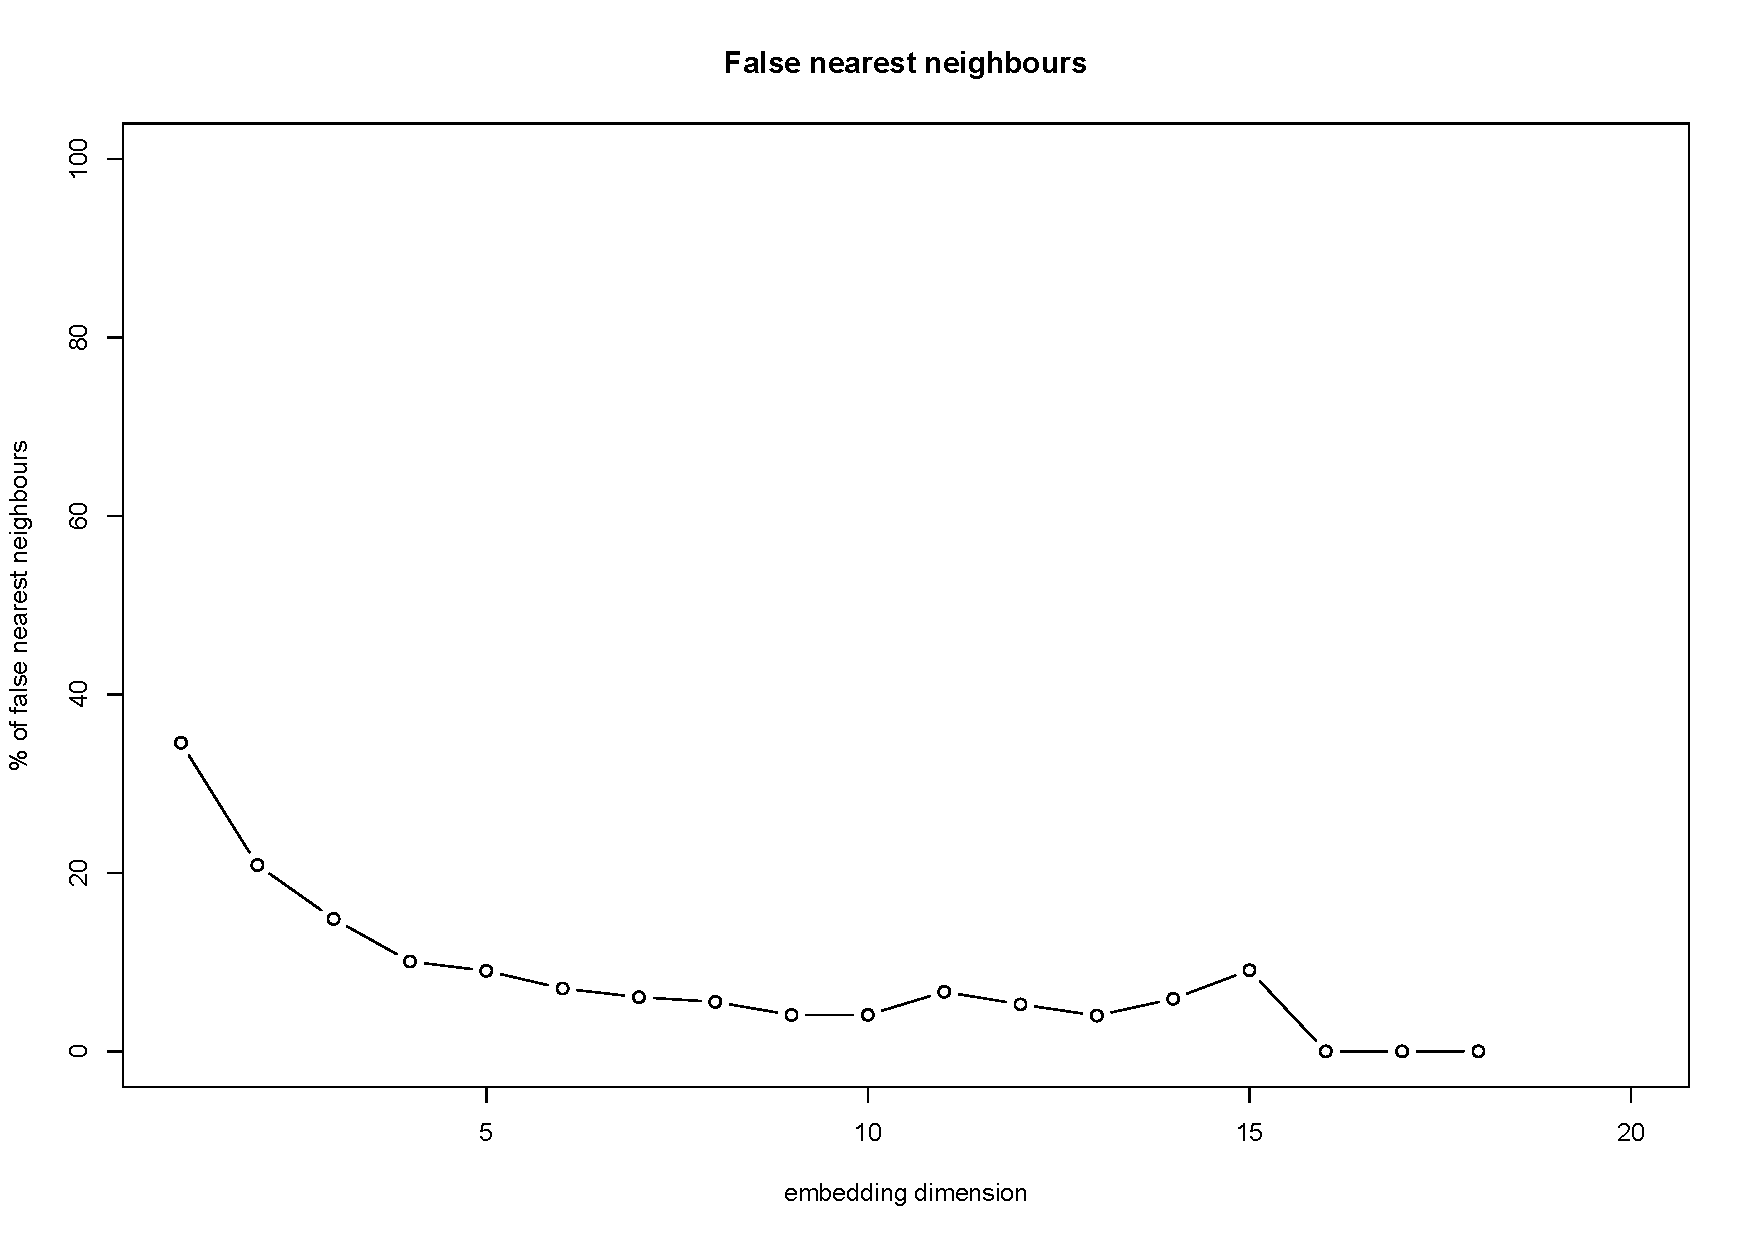
\includegraphics[width=\linewidth]{false_NN}
		\caption
		[Embedded dimensions optimization]
		{False nearest neighbours percentage as a function of the number of embedded dimensions.
			The x-axis show the considered numbers of embedded dimensions and the y-axis the percentage of false nearest neighbours.}
		\label{fig:false_nn}
	\end{minipage}	
\end{figure}
%
Following that, the radius was calculated in two steps (see \cref{alg:radius_opt}).
First, the goal \ac{rr} and a list of potential radii were initialized.
Here, the goal \ac{rr} was set to \SI{10}{\percent}, which is relatively high (e.g., compared to \SIrange{2}{5}{\percent} in \citet{Coco2014crqa-r}).
Setting the goal \ac{rr} to a higher value results in a stricter optimization that will reward closer recurrences.
The potential radii were generated by evenly spreading 20 candidates from 0 to the maximum value that occurs in the time series.
Then, each radius, along with the already optimized delay and embedding dimensions, was used to perform a \ac{crqa}.
A stricter policy was introduced in this step as well, as only lines longer than \SI{1}{\percent} of the time series' entire length were counted, as opposed to the typical setup that considers lines of any length.
With an average length of \SI{37.5}{minutes}, this means that lines longer than 11 time units, compared to the a typical setup with the minimal length of two time units (e.g., as done in \citet{Borrie2019syncing}).
This ensured that only long-term recurrences were taken into account, and shorter, possibly more random effects, were filtered out.
% note: calculated by multiplying 37.5 minutes * 60 to get seconds, then divide by 2 since each time unit (slice) was 2 seconds and again divide by 100 to get one percent of it.
Finally, the candidate radius that results in the smallest absolute distance from the goal \ac{rr} was chosen to perform the \ac{crqa}.
The radius optimization is described in \cref{alg:radius_opt}.
The optimization processes of all three parameters were done separately for each interaction.
%
\begin{algorithm}[t]
	\addtocounter{myequations}{1}
	\setcounter{myequations}{13}
	\caption{\acs{crqa} radius optimization}
	\label{alg:radius_opt}
	\algorithmcaption
		{\emph{The higher $n$ is (\cref{line:num_cand}), the higher the chance of a \ac{rr} close to the defined \emph{desired RR}.Also note that since \ac{rr} represents percentage of values in the recurrence plot, 100 is its highest possible value.
		Therefore, and since the radii in $R$ are traversed in increasing order, the search stops if this value is achieved(\cref{line:break_at_rr_100}).
		As explained in the text, in the presented studies $n = 20$ and $desiredRR = 10$ (see \citet{Coco2014crqa-r}).}}
	\DontPrintSemicolon
	\SetKwInOut{Input}{Inputs}
	\SetKwInOut{Output}{Output}
	
	\Input{\underline{$desiredRR$} -- the desired approximated \ac{rr} value\newline
		\underline{$optDelay$} -- the optimized delay\newline
		\underline{$optEmbedim$} -- the optimized embedded dimensions\newline
		\underline{$TS$} -- all values from both time series}
	\Output{radius producing \ac{rr} value closest to the defined desired \ac{rr}\newline}
	
	$n \gets$ number of radius candidates \label{line:num_cand}\;
	$R \gets \{r_i, \ldots, r_n\} : r_1 = 0, r_n = \max(TS)$\;
	$\forall r \in R : \lvert r_i - r_{i-1} \rvert = \lvert r_{i+1} - r_i \rvert$ \tcp*{evenly spread candidates}
	
	$candR \gets \varnothing$\;
	\ForEach{$r \in R$}{
		$currRR = crqa(ts_1, ts_2, optDelay, optEmbedim, \ldots\footnotemark).RR$ \tcp*{RR with candidate}
		$candR = candR \cup currRR$\;
		\uIf{$currRR = 100$}
		{\emph{break} \label{line:break_at_rr_100} \tcp*{\ac{rr} cannot be higher than 100}
		}
	}
	$optRadius = \displaystyle\argmin_{r \in R}(\lvert candR_r - desiredRR \rvert)$\;
\end{algorithm}
\eqname{Radius optimization algorithm for \acs{crqa}}
\footnotetext{As calculated by the \ac{crqa} package for R \citep{Coco2014crqa-r} with the additional arguments (unlisted in the algorithm itself) \emph{rescale=0, normalize=0, minvertline=length(ts1) / 100, mindiagline=length(ts1) / 100,} and \emph{tw=0}.}
%\todo{make sure algorithm block is on same page with its footnote and that the foot note is not cut into the next page}

\section{Dataset and feature extraction}
\label{sec:dataset_calls}

A collection of real-world calls with similar characteristics to those described in \cref{subsec:inside_sales} was used in this study.
These calls were all made by trained sales representatives and were aimed at high-stakes deals\footnote{In this case, around US\$100,000 each, as opposed to occasional mass calls to random people for selling small products where the losses are very small in comparison.
The reps in the calls collected here are aware of the deal scales and know that their performances are evaluated, pushing them to do their best in every single call.}.
To obtain a somewhat more homogeneous collection of conversations, calls of a single sales company (but multiple customer companies, see below) were selected.
Another constraint is that the collection comprises only calls from an early stage of the sales opportunity that is also the first encounter between the participating \ac{ae} and the prospect.
Therefore, behavior patterns that are not related to the history between the two interlocutors or the content of previous conversations between them can be identified.
Thus, these calls typically include a description by the prospects of their business' history, challenges and plans, followed by a demo by the sales person.
It is important to note that although every \ac{ae} prepares for such calls as part of the daily work, they are still spontaneous and in no way scripted.
%In some cases the prospect have already talked to an \ac{sdr} and/or communicated by email with the sales person.
%However, to the best of our knowledge, this is the first voice call with the prospect.
The calls in this collection were conducted using the Zoom platform, and were recorded automatically -- without any intervention from either side -- by Gong.io's system, which provides conversation intelligence services to said company.
Participants were notified of the recording, in compliance with all relevant laws and rights.
The calls were transcribed and diarized using an internal \ac{asr} system.

A single \ac{ae} and a single prospect participated in each call.
In total, 708 calls were used for analyses, each with a different customer company, with a total length of \SI{442}{hours} (mean 37.5 $\pm$15 minutes).
Furthermore, only calls longer than 15 minutes were selected, as shorter calls are often unsuccessful connection attempts or brief updates that are not representative for the desired conversation structure.
Call recording started immediately following the first greet from the prospect's side, and stopped when the meeting owner terminated it.
This eliminates segments during which one party is waiting for the other to join, and keeps only segments where both parties are present.
The 26 \acp{ae} (12 female) who participated in the calls formed 87 unique interlocutor pairs with different prospects.
Each prospect only ever spoke with one \ac{ae}.
The speakers on both sides were native speakers of American English.
For the purpose of this study, a call is defined as successful when a follow-up call under a more advanced stage is initiated or when an advancement in the opportunity is marked within one month.
These criteria follow common conventions of measuring call success\footnote{The benchmarks for successful deals are much more elaborate in practice and usually consider an entire selling process that comprises a series of calls.
However, many of those criteria are not relevant or cannot be enforced in the scope of this study.}.
This results in 51 calls (\SI{7.2}{\percent}) being defined as successful, which is within the industry standard ratio for this kind of calls.
Failed calls lasted on average 37 $\pm$15 minutes and successful calls 42 $\pm$16.5 minutes.
A two-sample Wilcoxon test \citep{Wilcoxon1945individual} between failed and successful call durations yielded a p-value of 0.04 with confidence level of \SI{95}{\percent}, confirming their differentiable distributions.
It goes without saying that the labels of both criteria are noisy, as sales opportunities might be lost because of parameters more related to the fit between the offered product and the prospect's needs, the available budget of the prospect, the presence of competitors, legal issues that tamper the deal etc.
To minimize such cases, calls done by personnel that are not sales people in the customer companies were filtered out.
%Following that, we hypothesized that successful sales calls would show more distinct speech patterns and vocal accommodation behaviors than unsuccessful calls.

As a preparation for the feature extraction and to increase temporal resolution, the audio signals were split into two-second slices (see motivation and further details in \cref{sec:analysis_hhci}).
Such fine-grained extraction makes the use of \ac{crqa} more elaborate, as it has more data points to consider (see \cref{sec:crqa}).
Splitting the turns also creates equal, consecutive, and more comparable time units for an interaction without introducing artificial boundaries by dividing it into a predefined number of parts.
The slicing was done per turn, so that a slice contains only the speech of a single speaker.
Any remainder of a turn got a slice of its own.
When a speaker is not speaking (e.g., during the turn of the other interlocutor), it is assumed that the last produced value is maintained until the speech is renewed and a new value can be measured.
This way, no discontinuities are created and the same number of data points is extracted for both speakers, which creates a better temporal representation of the conversation.
Feature extraction was done sequentially for all the conversations using Praat \citep{Boersma2001praat} scripts that extracted the \ac{f0} value from the middle of each slice and then post-processed the output to acquire cleaner measures.
Afterwards, the list of measures were turned into two equally long time series.
First, the values for each speaker were separated into two list.
Subsequently, missing values, e.g., due to non-speech slice, were replaced by the most recent valid value of their respective speaker, as motivated above.
Finally, if there were missing values at the beginning of a list, the first valid value of the that list was used, under the assumption that the first utterance represents the immediate time prior to it.
The resulting two lists had the same number of values representing the same timestamps along a single conversation, and were used for the \ac{crqa}.
Note that this process was performed individually for each conversation, regardless of whether one or more of the speakers participated in other conversations in the datatset.

\section{Analysis}
\label{sec:analysis_hhi}

Time series-based analysis methods like \ac{crqa} can be used in many ways.
The specific calculations used in this study are introduced below, followed by the results they yielded for the collection of sales calls and their interpretation.

\subsection{\Acs{crqa} output values}
\label{subsec:output_values}

Various measures can be computed based on a recurrence plot\footnote{See \citet{Marwan2007recurrence} and summary with additional measures in \url{http://www.recurrence-plot.tk/rqa.php}.}.
Some measurements deal with the \ac{los} and other diagonals across the plot while others consider vertical and horizontal lines.
Below are the definitions of some \ac{crqa} measurements used in this work.
For simplicity, it is assumed that the time series lengths are equal, so that $N_i=N_j=N$.

\begin{description}
	\item[\Acf{rr}] -- The percentage of recurrent points in the plot, i.e., the percentage of similar values between the two time series out of all the values.
	This corresponds to the correlation sum and defined as
	%
	\begin{equation}
		\label{eq:rr}
		RR = \frac{1}{N^2} \sum_{i=1}^{N_i} \sum_{j=1}^{N_j} R_{i,j}.
	\end{equation}
	\eqname{-- 4.4.5 CRQA-based measures: RR, DET, L, maxL, and ENTR}
	%
	This number generally corresponds to the overall colored area in the recurrence plot.
	The lengths of the time series ($N_i$ and $N_j$) are often -- but not necessarily -- equal
	
	\item[Determinism (DET)] -- The percentage of recurrences forming diagonal lines in the recurrence plot given a minimal length threshold $l_{\min}$.
	%
	\begin{equation}
		\label{eq:det}
		DET = \frac{\sum_{l=l_{\min}}^{N} l P(l)}{\sum_{l=1}^N l P(l)},
	\end{equation}
	%
	where $l$ is the length of a line and $P(l)$ is the histogram of the lengths $l$ of the diagonal lines.
	Note that $l=1$ refers to lines of length 1, i.e., a single recurrence point.	
	Similarly, $l=2$ are lines spanning over two time stamps (shortest length possible).
	This length is very forgiving in the case of accommodation, for such short lines can be formed arbitrarily and do not necessarily point to a meaningful accommodation process.
	Therefore, in the experiments presented here $l_{\min}$ was set to $\frac{N}{100}$, as in \cref{subsec:parameters_crqa}.
	
	Another measure, Laminarity (LAM), can be calculated the same way, but for the vertical lines in the plot.
	In that case, a $v_{\min}$ would be defined and $P(v)$ would provide the histogram of vertical line lengths.
	
	\item[Number of lines (NRLINE)] -- The total number of lines $N_l$ formed in the recurrence plot.
	In the context of accommodation, this is the number of accommodation \enquote{instances} between the two speakers lasting at least $l_{\min}$ time units.
	Also referred to as \emph{sustained recurrence} by \citet{Borrie2019syncing}, defined as the amount of alignment between conversational partners, where higher sustained recurrence values indicate higher amounts of sustained accommodation.
	As explained in the description of the measure \emph{DET}, only lines of length $\frac{N}{100}$ and longer were taken into account in the studies presented here to exclude \enquote{arbitrarily formed} diagonals.
	
	\item[Average length (L)] -- the average length of the diagonal lines, i.e., the average total accommodation time between the speakers.
	Higher value indicates longer average individual accommodation periods during the interaction.
	This is calculated by
	%
	\begin{equation}
		\label{eq:l}
		L = \frac{\sum_{l=l_{\min}}^N l P(l)}{\sum_{l=l_{\min}}^N P(l)}.
	\end{equation}
	%
	The average length of vertical lines, called trapping time (TT), is achieved in a similar way when using the same formula for the vertical line length and the histogram of vertical line lengths.
	
	\item[Maximal length (maxL)] -- The longest diagonal line in the plot, excluding the main diagonal.	
	This is the longest, uninterrupted time span over which accommodation between the speakers lasted.
	Higher value indicates a longer time span.
	The unit of this measure is the same as the axes of the plot (here, a representation of the conversation's turns).
	It is determined by
	%
	\begin{equation}
		\label{eq:maxl}
		L_{max} = \max_{l} (\{l_i; \ i=1, \ldots, N_l\}).
	\end{equation}
	%
	In a similar manner, the longest vertical line can be determined by traversing the vertical lines.
	
	\item[Entropy (ENTR)] -- The Shannon entropy of the probability distribution of the diagonal line lengths longer than the minimum length $l_{\min}$.
	Describes the variability of the amount of accommodation between the two speakers across the whole interaction.
	Higher value indicates more varied length of accommodation periods across the interaction.
	Shannon's entropy formula provides the value:
	%
	\begin{equation}
		\label{eq:entr}
		ENTR = -\sum_{l=l_{min}}^{N} p(l) \ln p(l),
	\end{equation}
	%
	where $p(l)$ is the probability of length $l$ from the lengths probability distribution.
	\item[Normalized entropy (rENTR)] -- The entropy value normalized by the number of lines formed in the recurrent plot.
	This measure helps understanding how the speakers vary across multiple calls with different characteristics.
\end{description}
%

\subsection{Results}
\label{subsec:results_hhi}

Since multiple variables are compared here, the Bonferroni correction \citep{Bonferroni1936teoria} was applied, so that the overall error rate across all variables is \num{0.05}.
Therefore, for a single comparison to be significant, it must be lower than $\alpha = 0.007$.
The non-parametric two-sample Wilcoxon test \citep{Wilcoxon1945individual} was used to determine the significance levels.
\cref{tab:crqa_results} shows a summary of means and p-values of the CRQA outputs for failed and successful calls.
The \ac{rr} mean value is about 10 in both groups, which proves to be a suitable goal for optimizing the parameters (see \cref{subsec:parameters_crqa}).
Significant differences between failed and successful calls were found for the values DET, NRLINE, and rENTR.
The first two, along with their higher means for the failed calls, indicate more time-synchronized convergence in the failed calls.
The latter is harder to interpret, especially due to the similar means for successful and failed calls.
It therefore seems that the behavior in both cases is evenly predicted -- but differently -- across calls.
One possible factor influencing these behaviors is related to the interlocutor leading the convergence effect, rather than the fact that it occurs at all.
The significant difference in the NRLINE measure stands in line with the findings in \citet{Borrie2019syncing}, supporting it as evidence for sustaining convergence in this study as well.
The same measures for measures were performed based on the leading speaker in each conversation (bottom part of the table), but no significant differences were found for this criterion.

\begin{table}[t]
	\caption{P-values of the two-sample Wilcoxon test comparing the \ac{crqa} output values based on call success/fail and leading speaker along with their respective mean values.
	See \cref{subsec:output_values} for details about each measure.
	Significant values based on the adjusted p-value threshold are set in bold.}
	\label{tab:crqa_results}
	\begin{tabularx}{\linewidth}{X
								 S
								 S[table-comparator=true, table-space-text-pre={$\ll$}]
								 S[table-comparator=true, table-space-text-pre={$\ll$}]
								 S
								 S
								 S
								 S}
		\toprule
						& {\thead{\acs{rr}}}	& {\thead{DET}} 		& {\thead{NRLINE}}		& {\thead{maxL}} 	& {\thead{L}} 	& {\thead{ENTR}} 	& {\thead{rENTR}} 	\\
		\midrule
		p (deal)		& 0.9					& \bfseries $\ll$0.001	& \bfseries $\ll$0.001	& 0.7 				& 0.07			& 0.1				& \bfseries 0.0058 	\\
		mean success	& 10.1					& 2.2					& 84.0					& 31.3 				& 17.8			& 1.4				& 0.8				\\
		mean fail		& 10.0					& 5.9					& 174.0					& 32.9 				& 15.3			& 1.5				& 0.8				\\
		\rule{0pt}{4ex}\\
		p (lead)		& 0.7					& 0.1					& 0.05					& 0.18				& 0.9			& 0.07				& 0.55				\\
		mean \acsp{ae}	& 10.0					& 6.1					& 186.7					& 35.2				& 15.2			& 1.5				& 0.8				\\
		mean prospects	& 10.1					& 5.4					& 154.4					& 31.2				& 15.7			& 1.4				& 0.8				\\
		\bottomrule	
	\end{tabularx}
\end{table}

To shed more light on the lead role in a conversation, \acl{cc} was used to determine which interlocutor leads the change in behavior.
As shown in \cref{fig:crqa_plot}, \ac{crqa} reports at which points in time the speakers were more inclined to be closer to each other.
As an extension, \acl{cc} finds the degree to which two time series are synchronized at different points in time.
For each such point, called \emph{lag}, the \acl{cc} function evaluates the correlation between the time series.
By iterating over a set of time points, the shift needed to make the time series maximally correlated can be found.
If this lag is positive, the first time series needs to be shifted forward to achieve maximal correlation, and vice versa.
In the context of convergence, \acl{cc} calculates the direction of the shift, which indicates the speaker leading the change.
The \acl{cc} function was not limited to a specific range of shifts, so that all possible lags were examined.
The lag associated with the maximal correlation, and only it, was used to determine the leader.
Since the calls in the collections used here have a typical structure, it is also interesting to see at which point of the conversation the maximal correlation occurs.
\cref{fig:barplot_conv_leaders} shows the time, in percent, in which the maximal correlation occurred for \acp{ae} and prospects in successful and failed calls.
The difference between the lag position distribution of reps and prospects is significant ($p = 0.0065$ with $\alpha = 0.05$).
However, the differences between successful and failed calls within the leading speakers are not significant.
It is also evident that when the reps were leading, they consistently did so at an early stage of the conversation, all the more so in successful calls, whereas the prospects' lead varied much more and generally happens at a much later time.
%
\begin{figure}[H]
	\centering
	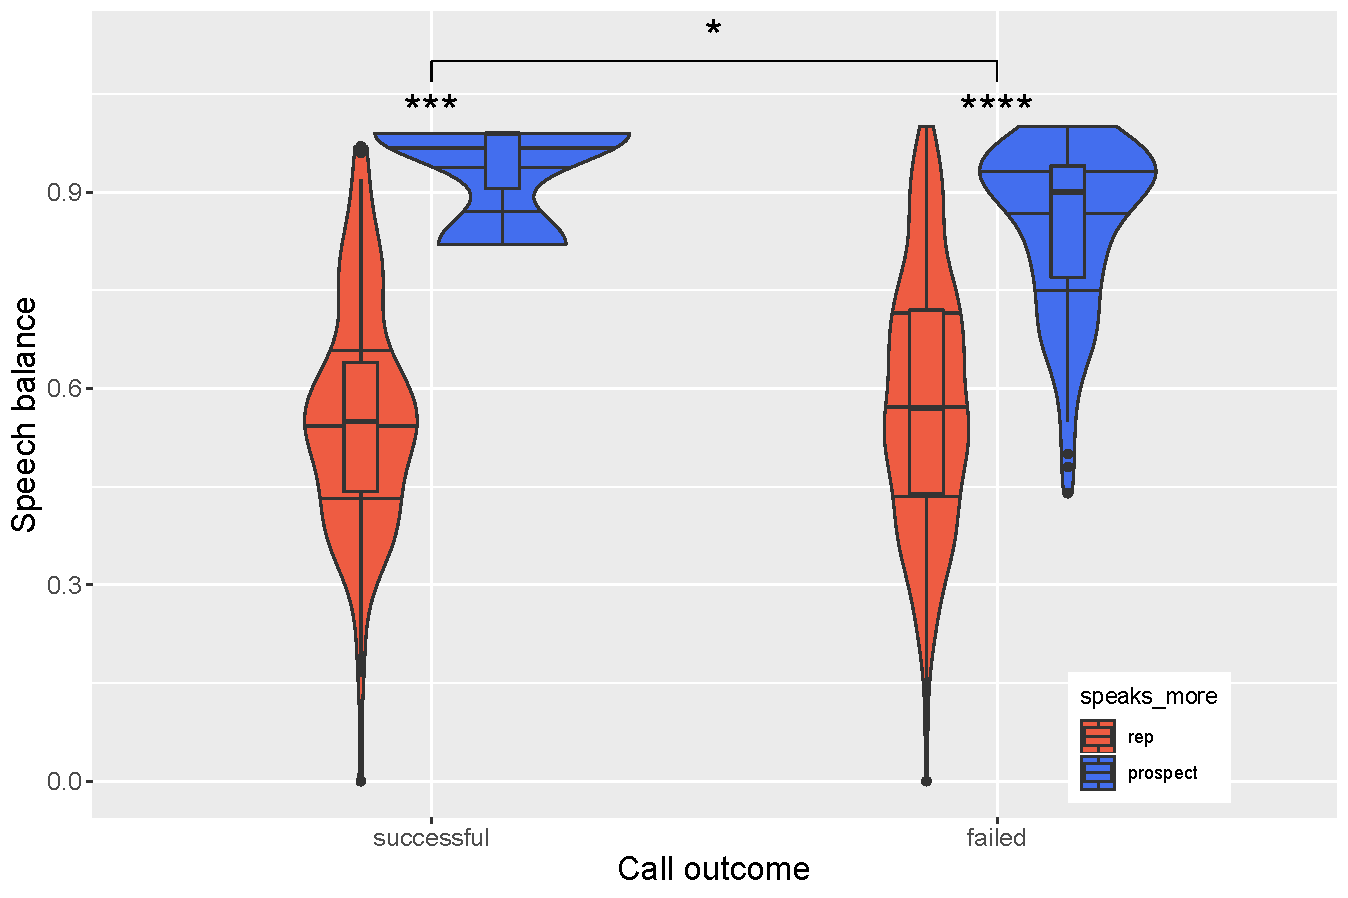
\includegraphics[width=\linewidth]{speech-balance_success_violin}
	\caption[Distribution of speech balance in successful and failed calls]
		{Comparison of speech balance distribution in successful and failed calls, sub-grouped by the speaker who spoke in total in individual calls (sales rep or prospect).
		The width of the shapes represent the probability density.
		The inner boxes show the central quartiles of the data with the median (excluding outliers) is marked by the thick horizontal line in it.
		The additional horizontal lines mark the \SI{25}{\percent}, \SI{50}{\percent}, and \SI{75}{\percent} quartiles of the data (including outliers).
		The asterisks stand the significance levels of the comparisons between the main groups (successful vs.\ failed) in the center and for the subgroups below it (* $p < 0.05$, *** $p < 0.001$, **** $p < 0.0001$)}.
	\label{fig:speech-balance_success_violin}
	\todo[inline]{could be easier to read if the inner boxplots had white fill and the quartile lines would be different color or a bit thicker}
\end{figure}
%
Another known conversational element in sales calls is the talk time each of the speakers get.
\Acp{ae} are trained to let the prospects speak as much as possible.
This is known to give them better feeling during the call, and also give the reps more information and opportunities to understand what their customers want to talk about.
All in all, this is good practice for keeping the \emph{speech balance}, i.e., the ratio between the total amounts of time in which speaker talked during the call.
Beside speech balance, the frequency and timing of speaker switching also sheds light on the dynamics of the speakers' vocal behaviors.
While each speaker should get sufficient amount of time to talk, it is also important to take and give the floor to the other interlocutor.
Long monologues can make the listener lose concentration or lack of expression, which damages the interaction.
Therefore, the \emph{interactivity} of the speakers is important as well.
While speech balance informs about the overall amount of time each speaker talked, interactivity complements this by informing how often a speaker gave the floor to the conversation partner.
Despite not being a concrete phonetic features, these two speech-related properties do fit into the overall notion of vocal accommodation nonetheless.
An analysis of these two additional conversation-level properties is performed here.
Speech balance was measured by
%
\begin{equation}
	\label{eq:speech_balance}
	speech\_balance = 
	1 - \left| \frac{\displaystyle \sum_{\forall S \in S_A} dur(S) - 
						\sum_{\forall S \in S_B} dur(S)}
					{\displaystyle \sum_{\forall S \in S_A \cup S_B} dur(S)}
		\right|,
\end{equation}
\eqname{Speech balance in conversation}
\noindent
%
where $S_A$ and $S_B$ are the slices in which speaker $A$ and $B$ speak, respectively and the function $dur$ returns the duration of a slice or set of slides.
The yielded value between 0 and 1 measures the percentage of balance in term of speech times, with 1 standing for \enquote{perfect balance}, i.e., equal talking times for both speakers.
As mentioned above, overall speech balance only reveals part of the whole picture.
Another part of it is the interactivity in the conversation, which is here defined as
%
%\begin{equation}
%	\label{eq:interactivity}
%	interactivity = 
%	,
%\end{equation}
%\eqname{Interactivity in conversation}
%\noindent
%
the percentage of slices, in which speaker change occurred after a consecutive slice sequence longer than some threshold (here, 1) without such change.
Sequences below this threshold can be generally ascribed to backchanneling, which does not indicate speaker change.
Interactivity and speech balance were measure for a superset of the dataset presented in \cref{sec:dataset_calls}.
\cref{fig:speech-balance_success_violin} shows the speech balance scores of successful and failed calls.
On the one hand, it is clear that lower the balance the more likely it is that reps had more floor time.
The recommendation to avoid imbalance is reflected by the significant difference between balance distribution in successful and failed calls.
On the other hand, prospects are only likely to talk more when the balance score is high, even more so in successful conversations.
This evident by the highly significant differences in both sub-groups.
No significant influences of interactivity on call outcome were found, and only a weak correlation between speech balance and interactivity was found. % r=0.2
%
\begin{figure}[H]
	\centering
	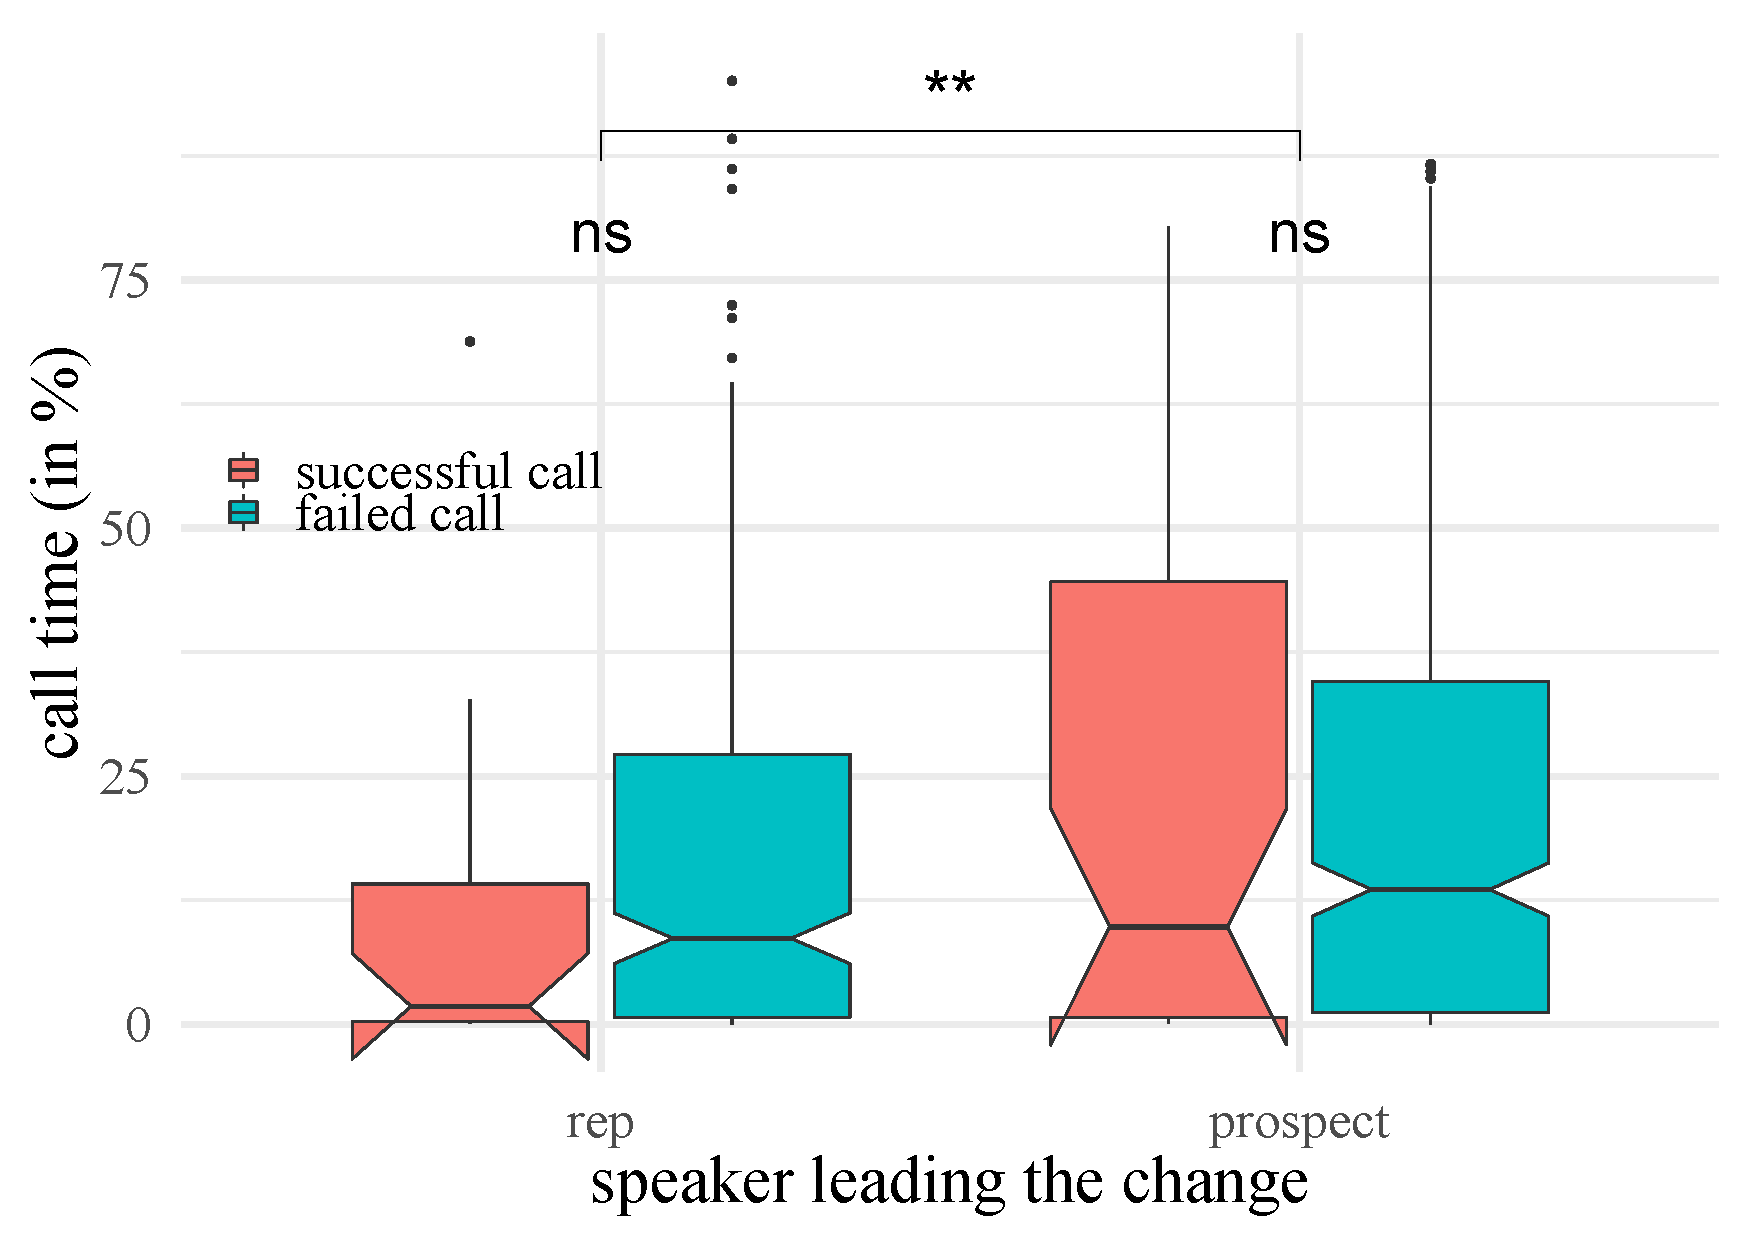
\includegraphics[width=\linewidth]{boxplot_ccf}
	\caption[Comparison between sales reps' and prospects' maximal \acl{cc} point in conversation for successful and failed calls.]
		{Comparison between the time of the call in which the maximal \acl{cc} occurs.
		The x-axis groups the calls based on the speaker, and the fill color further separates the calls to successful and failed ones.
		The y-axis points to the time in the call, in which the maximal correlation was detected.
		The horizontal lines within the boxes represent the median,
		the notches stand for the \SI{95}{\percent} confident level of the median, the area inside the boxes include the \acf{iqr} of values, the vertical lines outside the boxes show the value within the third quartile + 1.5$\protect\cdot$\ac{iqr}, and the isolated dots are the outliers.
		The significance level based on a Wilcoxon test comparing the two groups and their subgroups is given above the boxes.}
	\label{fig:barplot_conv_leaders}
	%	\todo[inline]{use logarithmic y-scale?}
\end{figure}
%

\section{Discussion}
\label{sec:discussion_hhi}

The results of the study show two sides of \ac{crqa} with respect to call success and role detection.
On the one hand, successful and failed calls could be distinguished by three of the \ac{crqa} output values.
Although based on \ac{hhi} studies it might be hypothesized that recurrence is more likely to occur in successful calls, the means of two of the three values suggest the opposite.
Yet, this stands in line with some studies from sales research that show more \enquote{desperate} behavior from the rep side when a call seems to fail.
This includes unconsciously showing assimilation towards the prospect, and over-emphasizing the deal's \ac{roi}, with the hope that it will convince the prospect to buy \citep{Orlob2018roi}.
However, these often achieve the opposite effect and are therefore discouraged in the sales industry.
Another possible explanation is that reps give up their own lead in the call (see below) when a call is on the verge of failing, and instead let the prospects lead, either as a natural tendency or to give them a better feeling.
This, too, is a known effect in sales business.
On the other hand, utilizing \acl{cc} lags (i.e., how the recurrence needs to shift for the speakers to be maximally aligned) was useful for differentiating between the leader in the calls.
When \acp{ae} lead, they tend to do so at an earlier stage than prospects, especially in successful calls.
This, together with the \ac{crqa} results shown in \cref{subsec:results_hhi}, suggests that \acp{ae} do not necessarily always lead the conversation, but know when to exploit this technique, consciously or not, to improve their stance in calls.

Though beyond the scope of this work, three further investigation directions on this topic are suggested here:
First, deepening the aspect of the relationship between the \acp{ae} and the prospects by examining the mutual changes not only within single calls, but over the course of an entire deal spanning over several meetings.
This could shed light on long-term changes and connect changes to the success of the deal.
Secondly, distinguishing between different \acp{ae} to find behaviors of sub-groups or identifying star reps.
For example, sales persons with higher ratings might be revealed to better exploit accommodation and trigger different behavior on the prospect side to increase their chance of closing a deal.
Lastly, different methods could be applied to predict the success of a call.
Specifically, machine learning methods that are good at capturing serial changes, such as recurrent neural networks, can be used to train such prediction models.
All of these direction can also be combined with more features to uncover more consistent accommodation patterns.

% Conclusion
%We have presented a study that examines phonetic accommodation in real-world sales calls.
%The focus was on mutual proximity of \acl{f0} between sales persons and prospects to find both how close they are to each other in general across the call, and how quickly changes in proximity occur and by whom they are initiated.
%This was done by \acf{crqa} and \aclp{cc}, which together provide various measures regarding recurrence between the speakers and who leads the other in terms of \acl{f0} changes.
%A corpus of 708 calls was used for the analyses, which makes it possible to find more global, consistent effects that are not influenced by the design of a specific experimental setting.
%The results show significant differences in some of the values between successful and failed calls, and significant differences between the leading behavior of sales persons and prospects.
%These findings encourage further investigations, like looking for other predictors of successful calls and examining the influence of additional features and factors on the success of calls.
